\subsubsection{Proceso propuesto}

El proceso propuesto se modela en BPMN 2.0 como contraparte de los diagramas del Objetivo 1 (Figuras~\ref{fig:bpmn1}, \ref{fig:bpmn2} y \ref{fig:bpmn_comunicacion}). Se presentan dos diagramas: el ciclo completo de atención con el sistema y la comunicación con el paciente mediante el agente conversacional.

\paragraph{Ciclo completo de atención con el sistema}

El sistema reemplaza las Etapas 1 y 2 por un único flujo. La información se registra una sola vez durante la atención, a cargo del odontólogo, y la secretaria se limita al registro de llegada, a la filiación de pacientes nuevos, al cobro y al agendamiento. La Figura~\ref{fig:ob2_tobe_atencion} modela el flujo con los carriles Paciente, Secretaria y Odontólogo/a, con las siguientes actividades:

\begin{enumerate}[leftmargin=*]
    \item \textbf{Llegada y filiación.} La secretaria registra la llegada del paciente en la agenda centralizada. Si no tiene cita, se crea una en un horario libre. Para un paciente nuevo, registra sus datos de filiación. Los antecedentes ya no se toman en recepción.

    \item \textbf{Apertura y registro clínico.} El odontólogo abre la atención, revisa el historial del paciente y registra la anamnesis, los antecedentes y el odontograma por pieza y cara.

    \item \textbf{Tratamiento, diagnóstico y receta.} El odontólogo registra el diagnóstico CIE-10 y los procedimientos desde los catálogos. Si se requiere medicación, genera la receta desde el catálogo y la imprime para su firma.

    \item \textbf{Cierre.} El odontólogo cierra la atención. Los tratamientos y valores quedan disponibles para el cobro.

    \item \textbf{Cobro.} La secretaria cobra y registra el abono. El saldo se calcula automáticamente.

    \item \textbf{Agendamiento.} Si se requiere, la secretaria asigna la siguiente cita en la agenda centralizada.
\end{enumerate}

\afterpage{%
\begin{landscape}
\begin{figure}[H]
    \centering
    \IfFileExists{img/ToBe_Atencion.pdf}{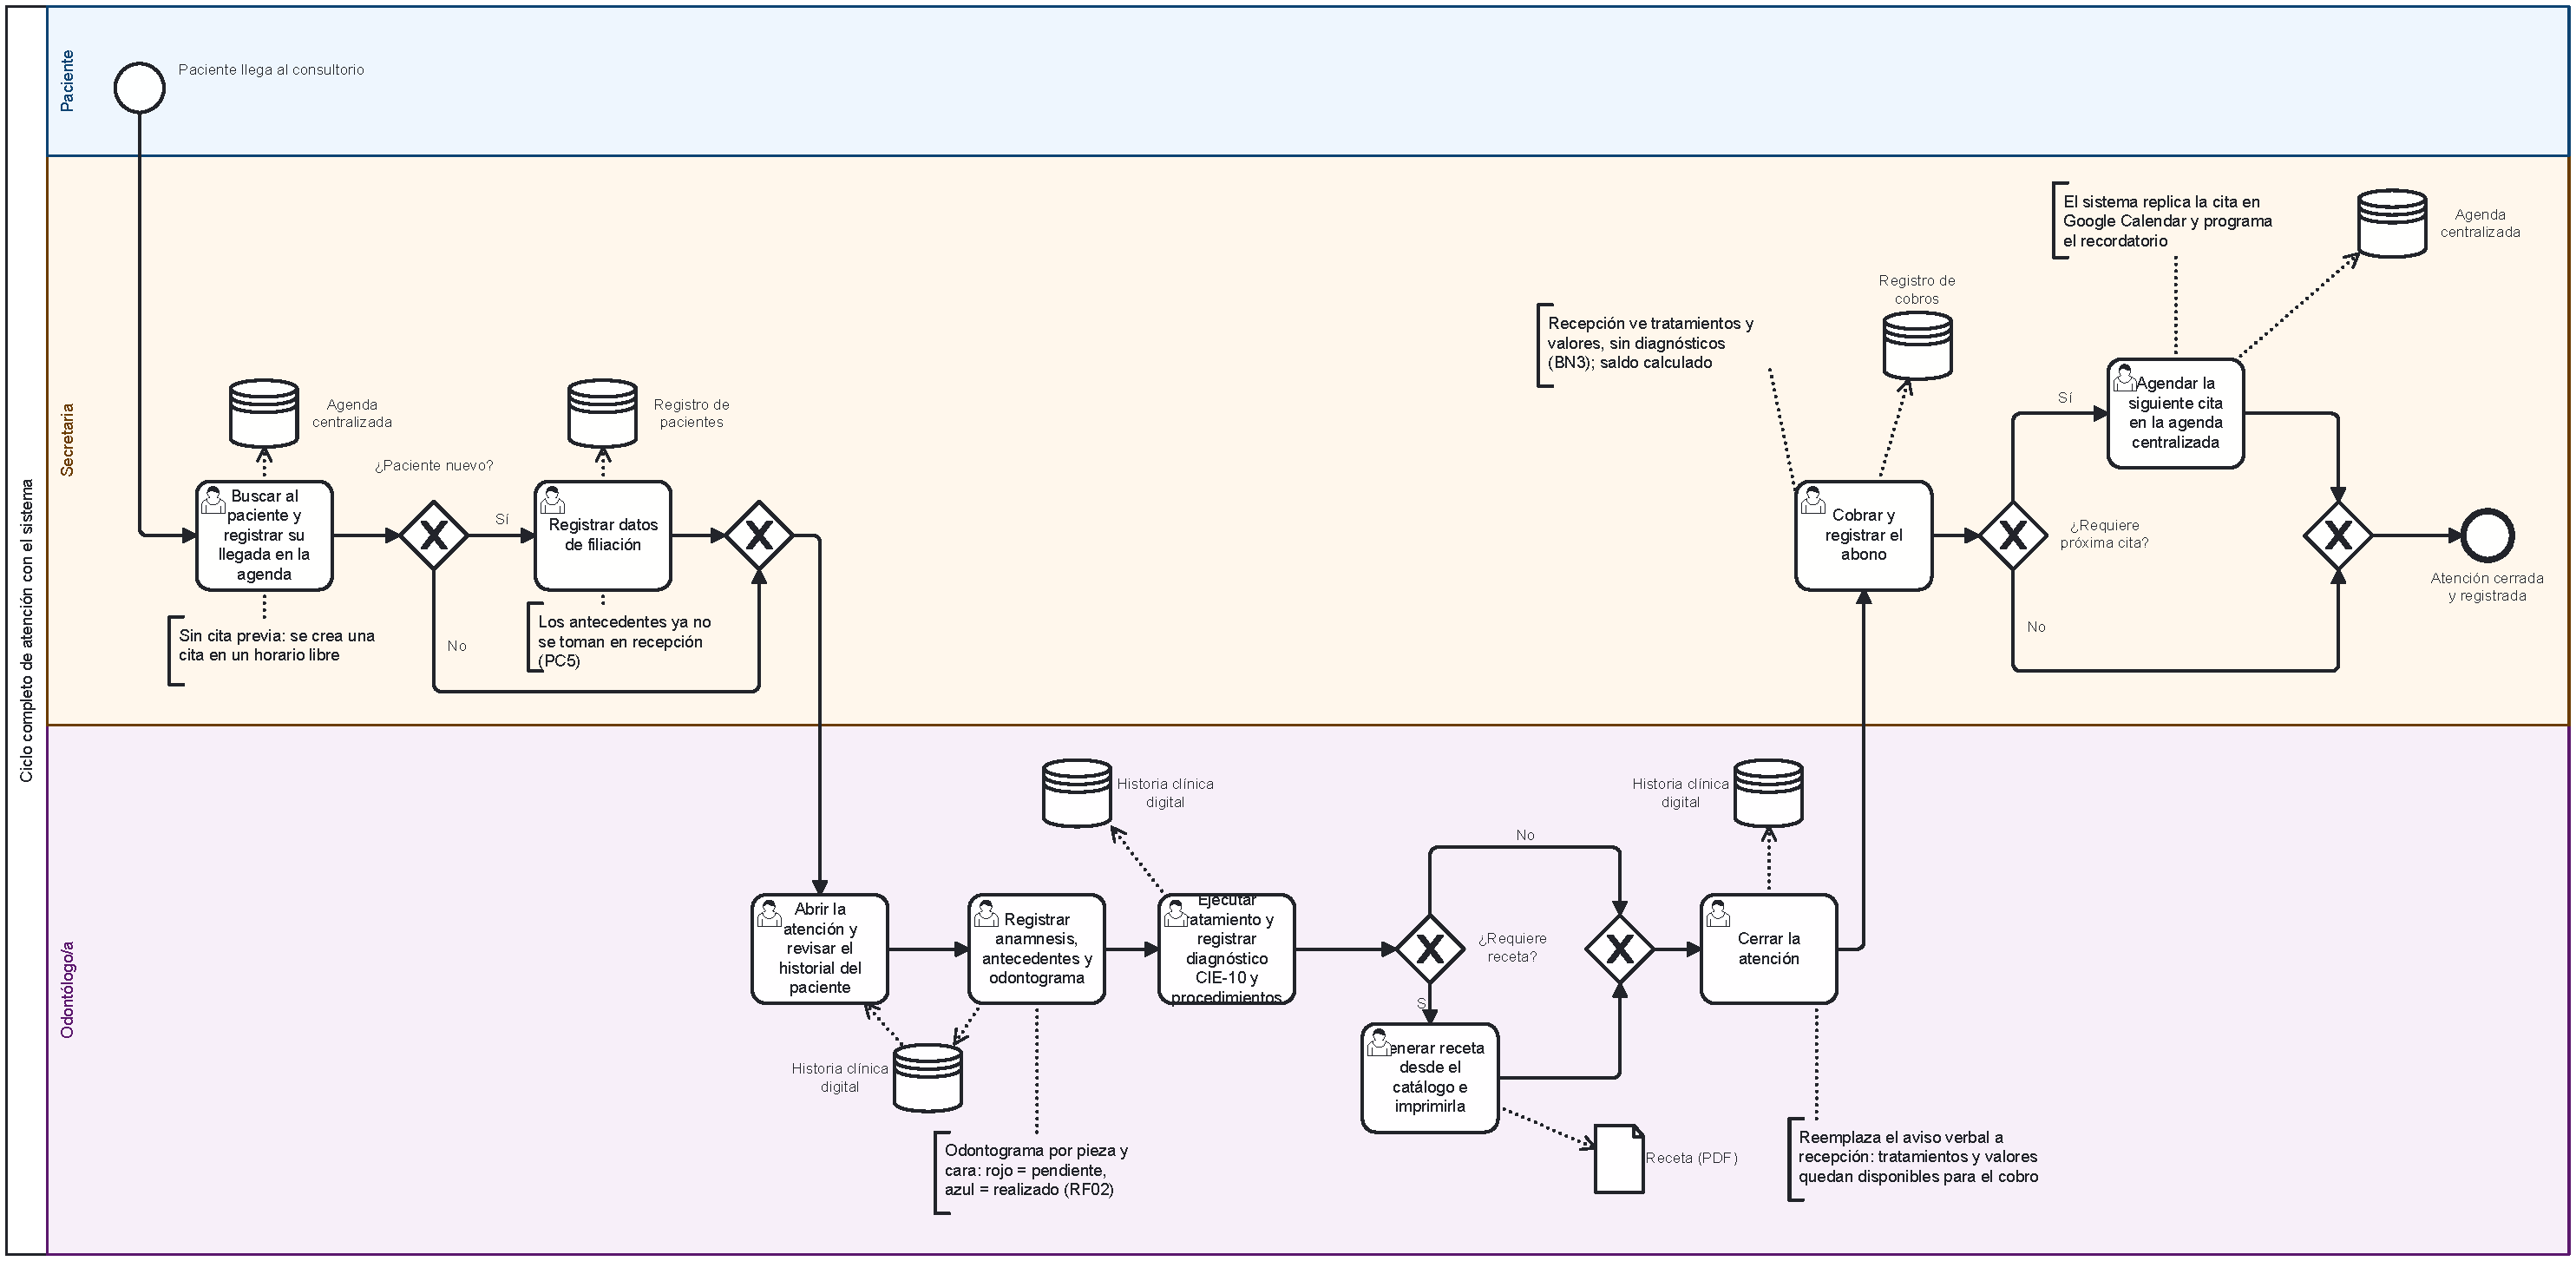
\includegraphics[width=\linewidth,height=0.85\textheight,keepaspectratio]{img/ToBe_Atencion.pdf}}{\fbox{\parbox{0.9\linewidth}{\centering Pendiente: exportar diagramas/bpmn/ToBe\_Atencion.bpmn a img/ToBe\_Atencion.pdf}}}
    \caption{Ciclo completo de atención con el sistema propuesto}
    \label{fig:ob2_tobe_atencion}
\end{figure}
\end{landscape}
}

En el diseño se elimina la Etapa 2: la historia clínica digital, con los campos del Formulario 033, queda registrada al cerrar la atención, por lo que la transcripción de la ficha rápida y la preparación de fichas del día siguiente dejan de ser necesarias. La secretaria no edita datos clínicos (BN3) y solo ve los tratamientos y sus valores para el cobro (RNF01).

\paragraph{Comunicación con el paciente mediante el agente conversacional}

Las Figuras~\ref{fig:ob2_tobe_comunicacion_p1} y~\ref{fig:ob2_tobe_comunicacion_p2} modelan la comunicación con el paciente mediante un agente conversacional, con los carriles Paciente, Agente conversacional, Secretaria y Odontólogo/a. El agente ejecuta tareas automáticas de servicio. El paciente escribe libremente o elige una opción del menú; el flujo no cambia. Por su extensión, el modelo se divide en dos partes: (1) acceso, consulta general y solicitud de cita; (2) confirmación de citas y derivación, que parte de las consultas derivadas de la primera. El flujo se agrupa en cuatro categorías:
\begin{itemize}[leftmargin=*]
    \item \textbf{Acceso y consulta general.} El agente muestra el aviso de privacidad en la primera interacción y registra la aceptación explícita (RF09). Responde horarios, precios y formas de pago sin intervención del personal (N1).

    \item \textbf{Solicitud de cita.} El agente identifica al paciente por su teléfono y, si está registrado, ofrece horarios disponibles y registra la cita en la agenda centralizada (RF11, RF12, N2). Las citas solicitadas por otro canal las registra la secretaria o el odontólogo en la misma agenda (N4).

    \item \textbf{Confirmación de citas.} El día previo, el agente envía un recordatorio con las opciones Confirmar, Cancelar o Reprogramar (RF14, N3). Sin respuesta, la cita queda sin confirmar y visible para recepción.

    \item \textbf{Derivación.} Las consultas clínicas, de saldo o no reconocidas se derivan al personal (RF13, N5).
\end{itemize}

\afterpage{%
\begin{landscape}
\begin{figure}[H]
    \centering
    \IfFileExists{img/ToBe_Comunicacion_P1.pdf}{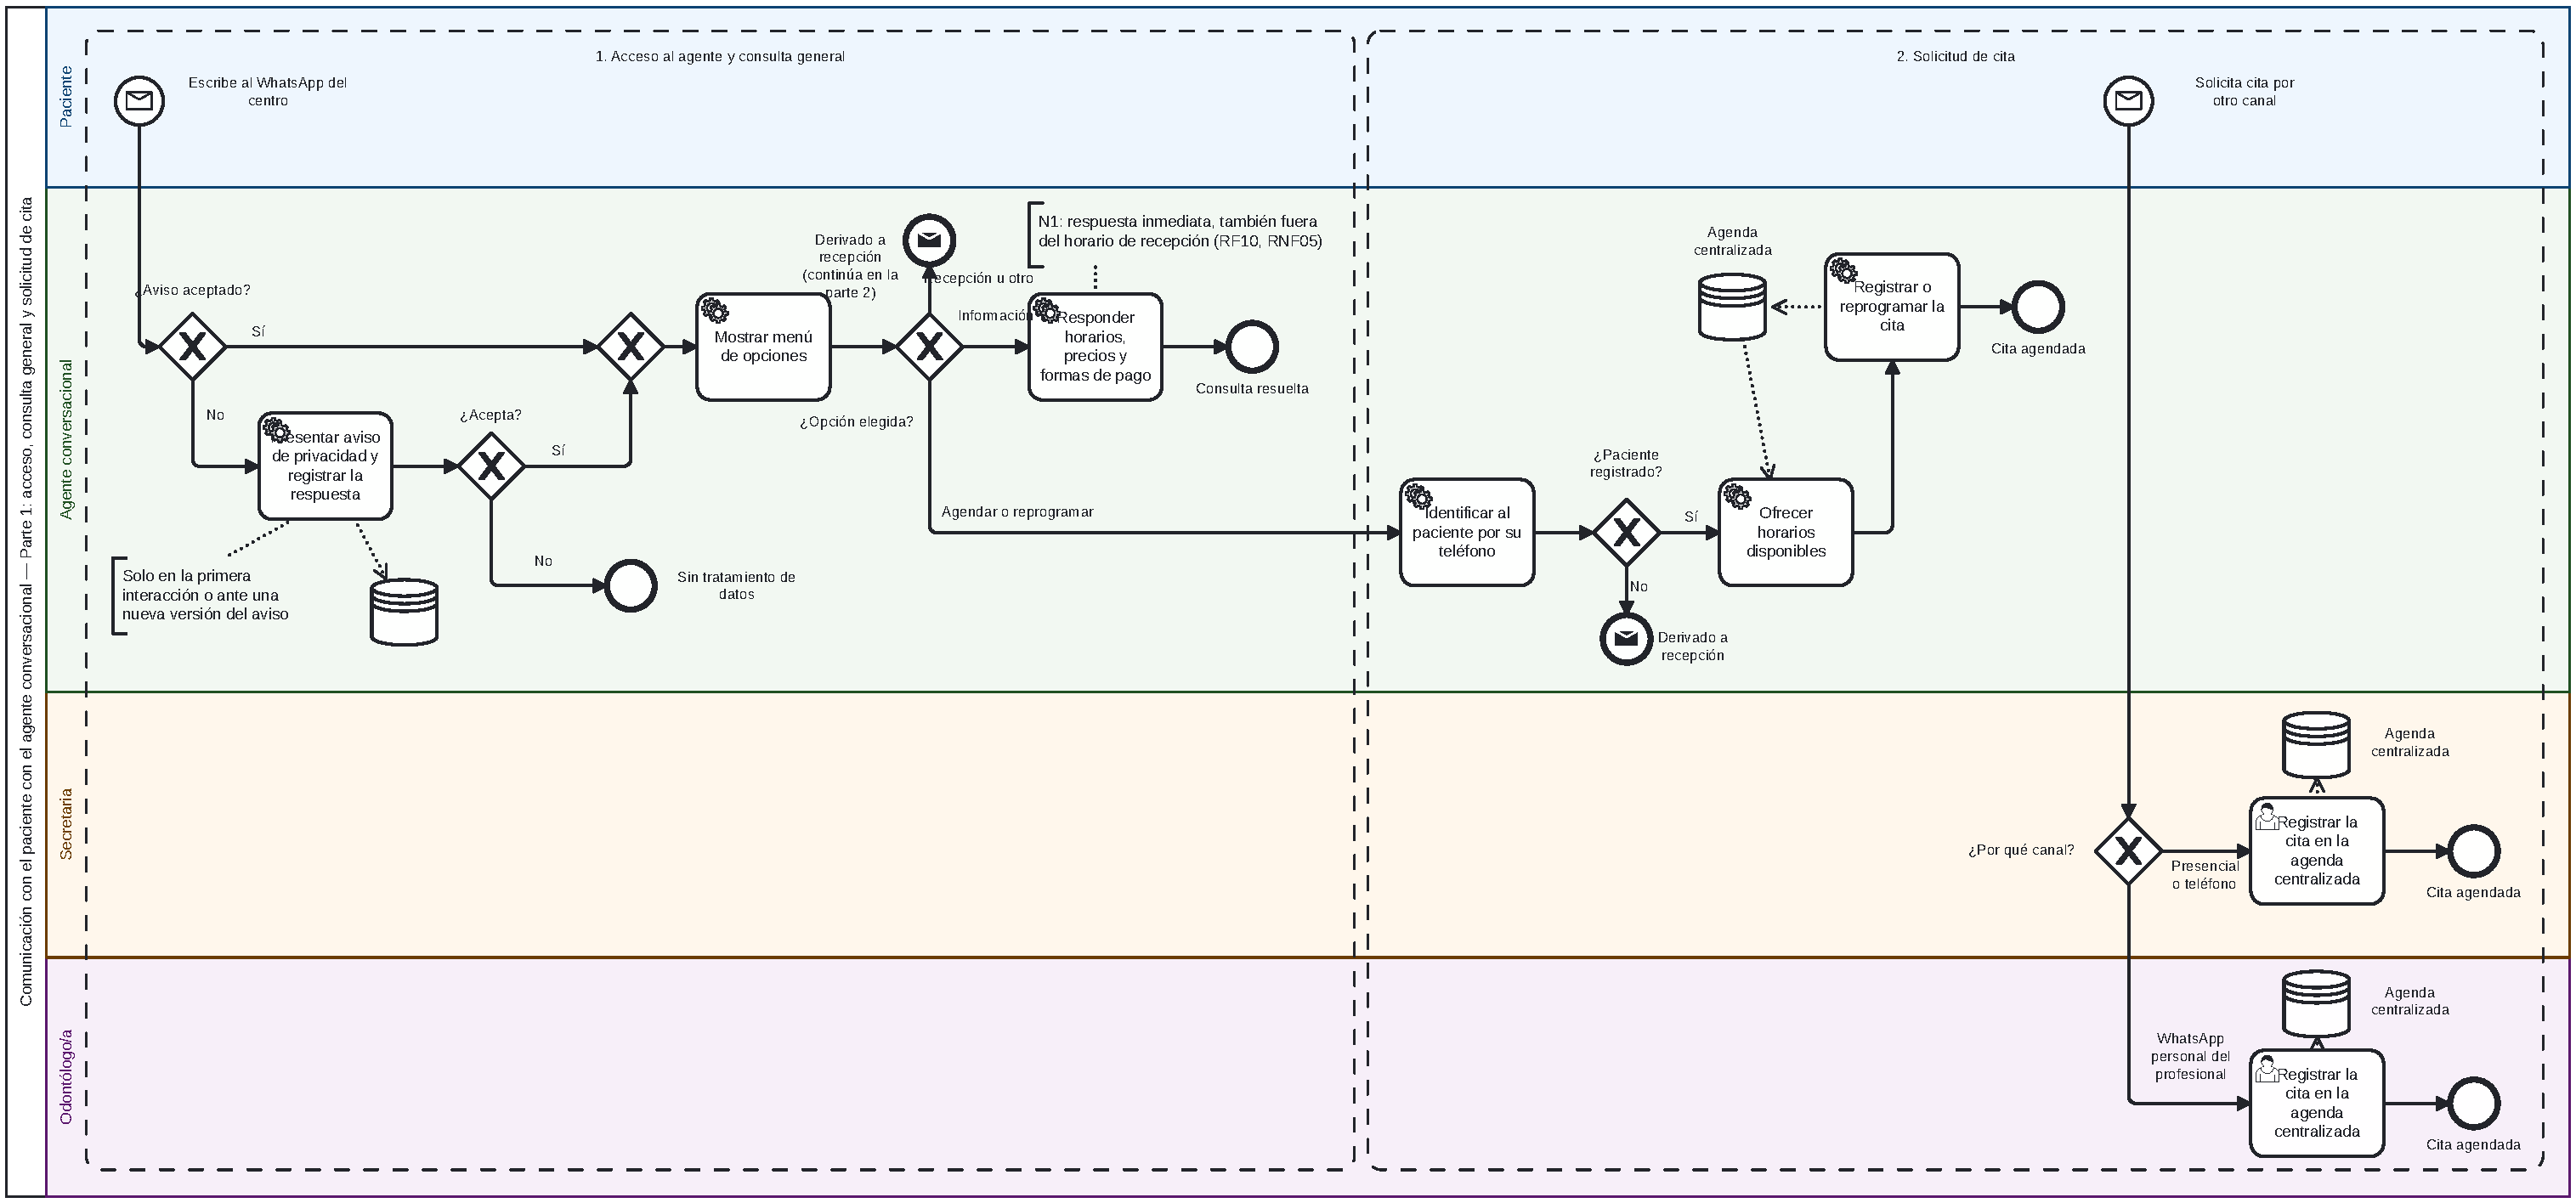
\includegraphics[width=\linewidth,height=0.85\textheight,keepaspectratio]{img/ToBe_Comunicacion_P1.pdf}}{\fbox{\parbox{0.9\linewidth}{\centering Pendiente: exportar diagramas/bpmn/ToBe\_Comunicacion\_P1.bpmn a img/ToBe\_Comunicacion\_P1.pdf}}}
    \caption{Comunicación con el paciente mediante el agente conversacional, parte 1: acceso, consulta general y solicitud de cita}
    \label{fig:ob2_tobe_comunicacion_p1}
\end{figure}
\end{landscape}

\begin{landscape}
\begin{figure}[H]
    \centering
    \IfFileExists{img/ToBe_Comunicacion_P2.pdf}{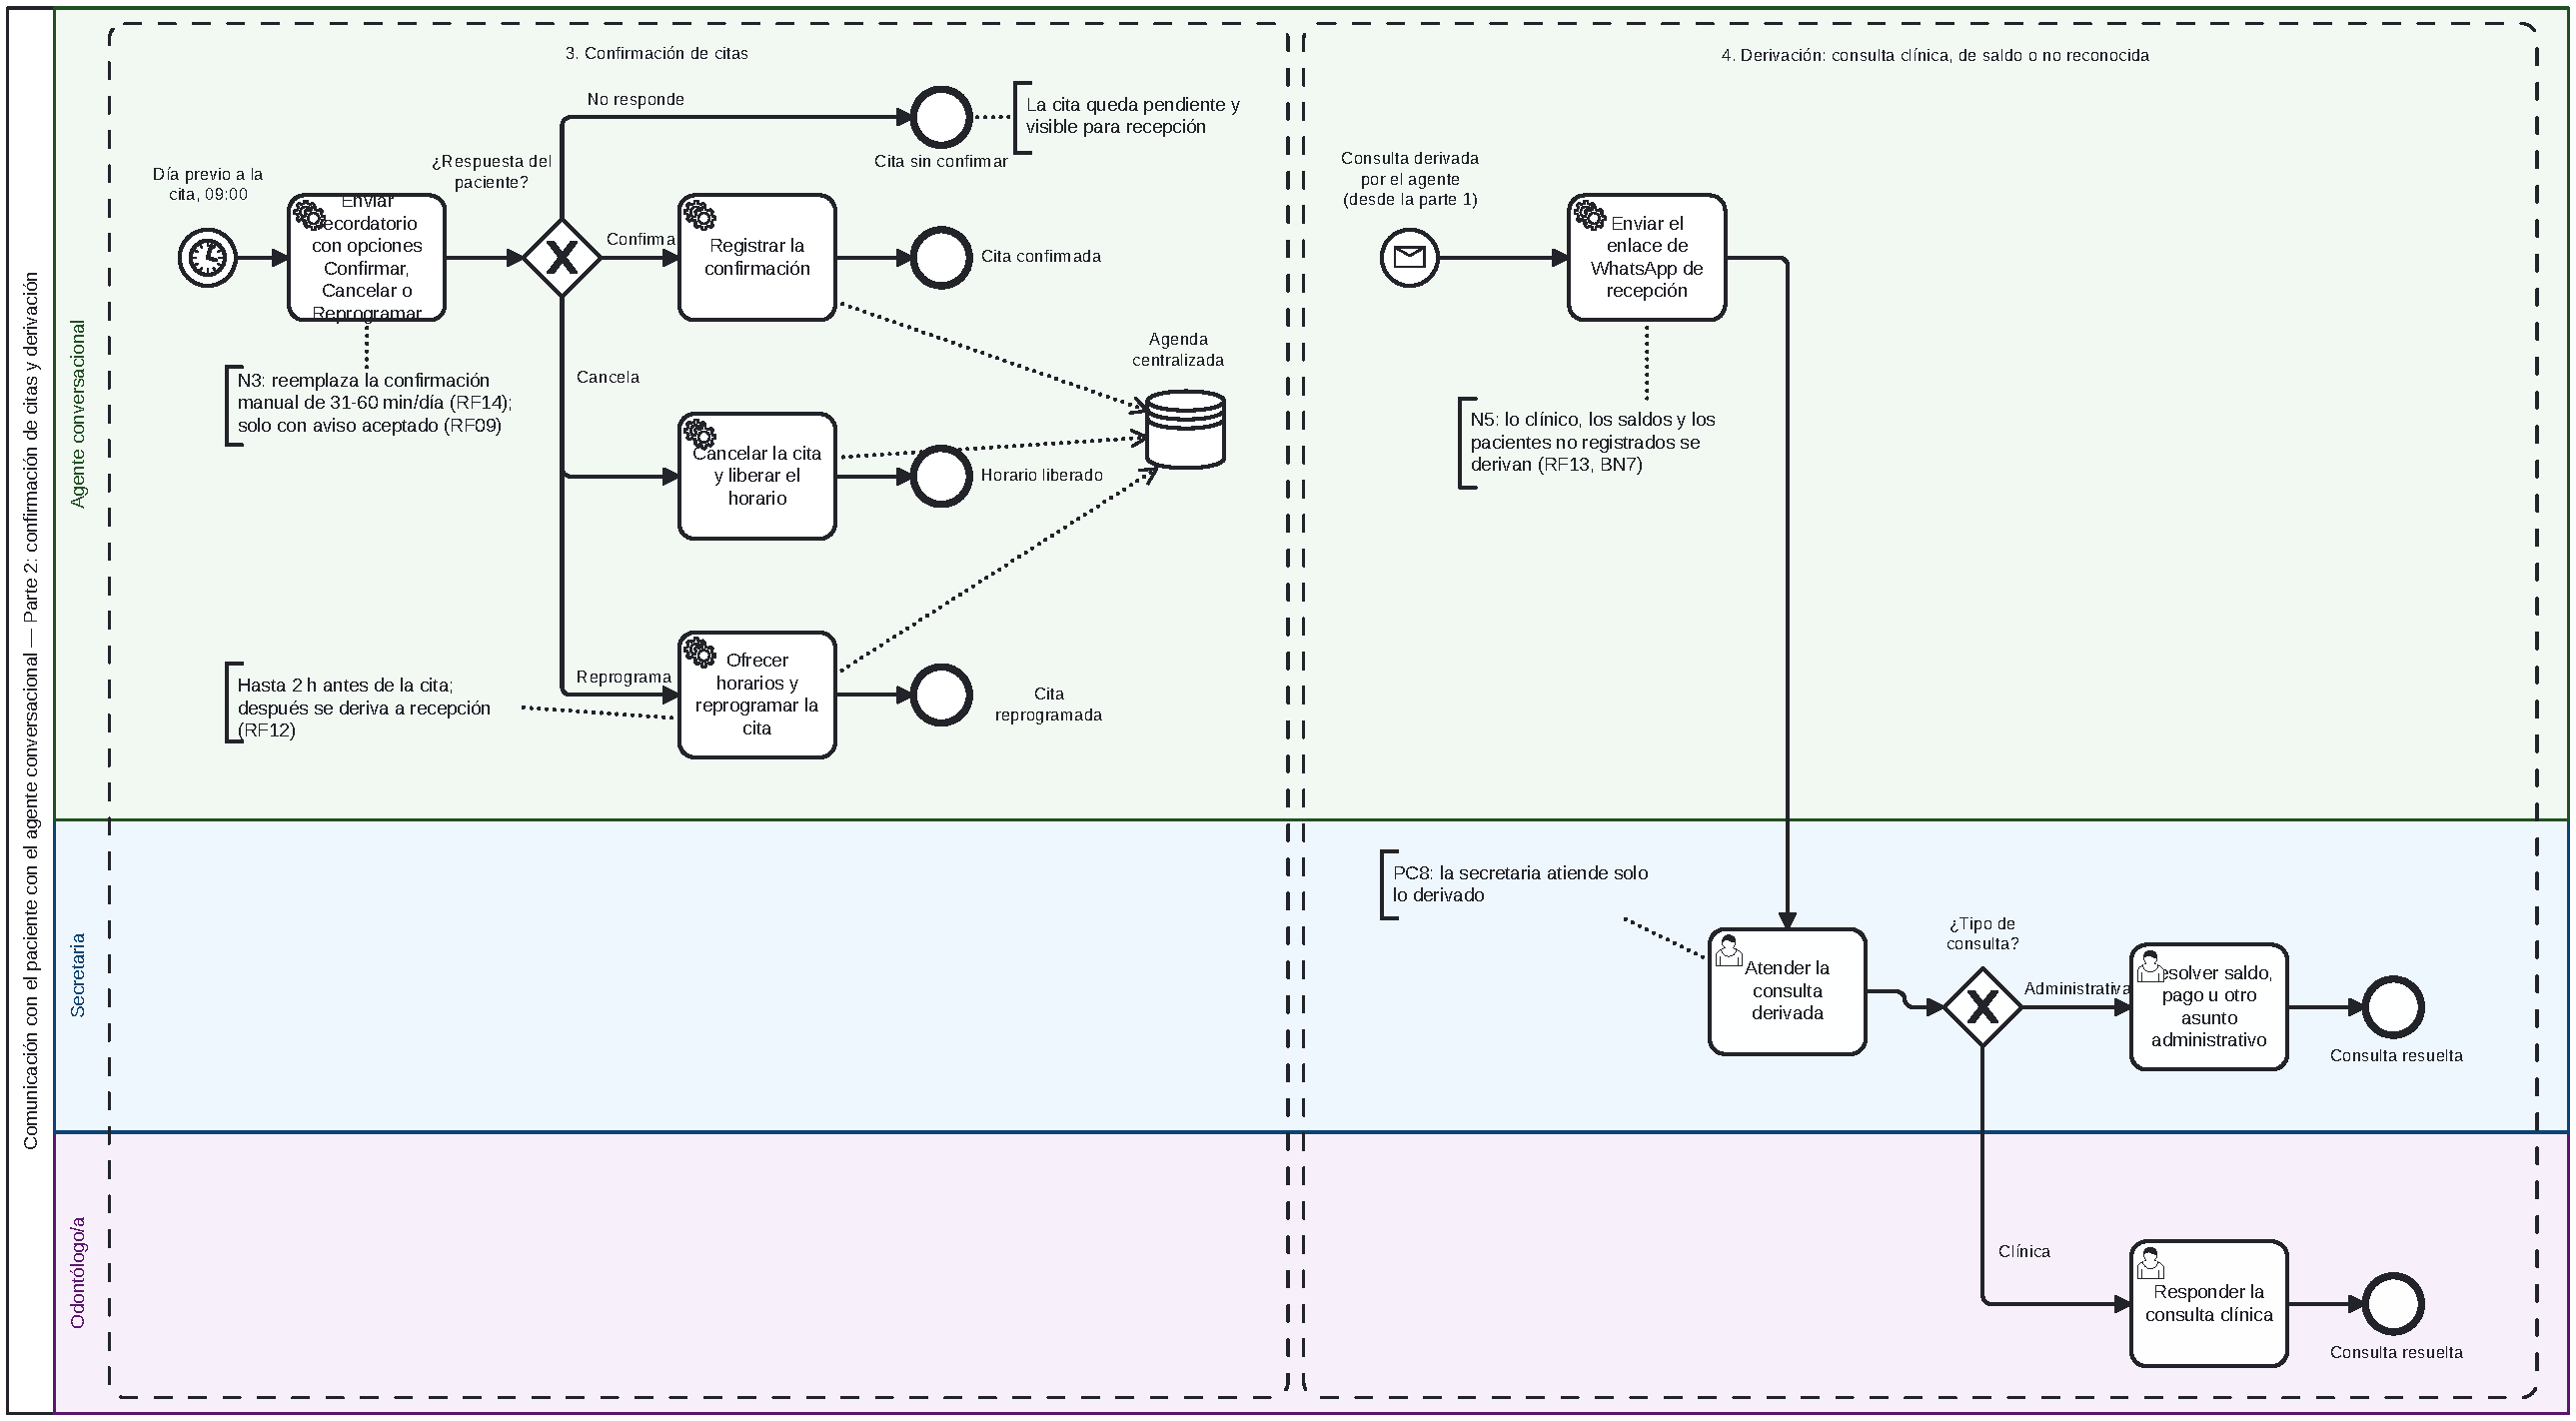
\includegraphics[width=\linewidth,height=0.85\textheight,keepaspectratio]{img/ToBe_Comunicacion_P2.pdf}}{\fbox{\parbox{0.9\linewidth}{\centering Pendiente: exportar diagramas/bpmn/ToBe\_Comunicacion\_P2.bpmn a img/ToBe\_Comunicacion\_P2.pdf}}}
    \caption{Comunicación con el paciente mediante el agente conversacional, parte 2: confirmación de citas y derivación}
    \label{fig:ob2_tobe_comunicacion_p2}
\end{figure}
\end{landscape}
}

Los efectos del proceso propuesto sobre el $TGA$ son hipótesis de diseño: se espera que $T_4$ y $T_5$ desaparezcan, lo que retira 7,32 de los 13,62 min, y que $T_1$ a $T_3$ disminuyan. El Objetivo 3 compara ambos procesos midiendo los mismos tramos.
